\pagestyle{empty}

\definecolor{plop}{HTML}{4D7186}
\begin{textblock}{1}(0,0)
    \noindent\textcolor{plop}{\rule{\paperwidth}{.55\paperheight}}
\end{textblock}


\begin{textblock}{1}(0,.55)
    \noindent\textcolor{black}{\rule{\paperwidth}{.45\paperheight}}
\end{textblock}


\begin{textblock}{1}(.1,.09)
    \noindent{\fontsize{24.88}{2}\selectfont
        \bfseries\textcolor{white}{Note}}
\end{textblock}

\begin{textblock}{1}(.1,.15)
    \noindent {\fontsize{24.88}{2}\selectfont
    \bfseries\textcolor{white}{电磁场与微波技术}}
\end{textblock}

% \begin{textblock}{1}(.1,.21)
%     \noindent{\fontsize{30}{2}\selectfont
%         \bfseries\textcolor{white}{for \LaTeX}}
% \end{textblock}

\begin{textblock}{1}(.1,.45)
    \noindent {\fontsize{20.74}{2}\selectfont
        \bfseries\textcolor{white}{hyq}}
\end{textblock}



\begin{textblock}{.9}(.05,.56)
    \begin{flushright}
        \noindent {\fontsize{20.74}{2}\selectfont
            \bfseries\textcolor{orange}{version 1.1}}
    \end{flushright}
\end{textblock}


\begin{textblock}{.45}(.5,.82)
    \begin{center}
        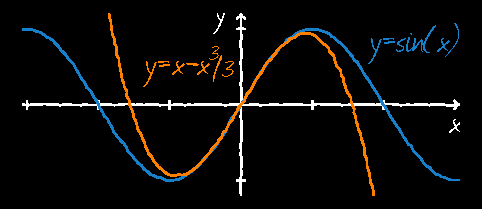
\includegraphics[width=.45\paperwidth]{figure/titlepage/dlsin}
    \end{center}
\end{textblock}

\begin{textblock}{.4}(.05,.65)
    \begin{center}
        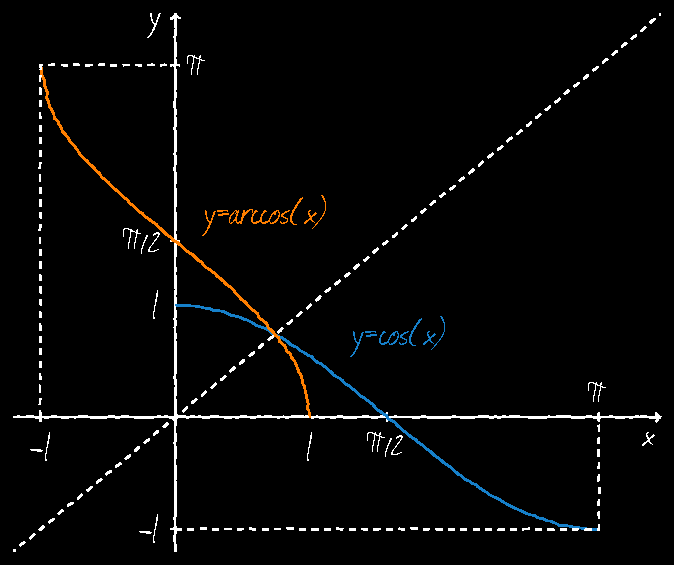
\includegraphics[width=.4\paperwidth]{figure/titlepage/arccos}
    \end{center}
\end{textblock}


\begin{textblock}{.6}(.05,.6)
    \noindent {\fontsize{20.74}{18}%
    \textcolor{white}{$u(z)=\frac{E_gZ_0}{(Z_g+Z_0)(1-\varGamma_g\varGamma_l \mathrm{e}^{-\mathrm{j}2\beta l})}\left( \mathrm{e}^{-\mathrm{j}\beta z} + \varGamma_l \mathrm{e}^{-\mathrm{j}2\beta l} \mathrm{e}^{\mathrm{j}\beta z}\right)$}}
\end{textblock}


\begin{textblock}{.4}(.4,.77)
    \noindent {\fontsize{17.28}{18}%
    \textcolor{white!80}{$\displaystyle 
    P_\mathrm{max}=\frac{E_\mathrm{max}^2ab\sqrt{\varepsilon_r}}{480\pi\xi}$}}
\end{textblock}

\begin{textblock}{.4}(.1,.93)
    \noindent {\fontsize{14.4}{18}%
    \textcolor{white!50}{$\displaystyle 
                \binom{n}{k} = \frac{n!}{k!(n-k)!}$}}
\end{textblock}


\begin{textblock}{.6}(.5,.69)
    \noindent {\fontsize{17.28}{18}%
    \textcolor{white!10}{$\displaystyle 
                \zeta_k = |a|^{1/n} \mathrm{e}^{i(\mathrm{arg}(a)+2k\pi)/n}$}}
\end{textblock}


\begin{textblock}{.3}(.75,.73)
    \noindent {\fontsize{17.28}{18}%
    \textcolor{white!10}{$\displaystyle \mathrm{e}^{i\pi}+1=0$}}
\end{textblock}



\null\newpage\pagestyle{nexus}